%%--------------------------------------------------
\subsection{Pedestrian Simulation}
\label{ss:Pedestrian Simulation}
%% - - - - - - - - - - - - - - - - - - - - - - - - -
CASSIA Framework can illustrate a trade-off structure of social problems.
The most of social problems like planning of evacuations from disasters
are not simple optimization problems but dilemmas among multiple
objective functions.
We will show an example to apply CASSIA Framework to find
such trade-off structures using evacuation planning for Nishiyogogawa-ku, Osaka,
which includes over 300 control parameters\cite{Noda2018b}.
Because of the large degrees of freedom,
the search space of this problem is so huge
that the solution of this problem require high-performance
computing like K-computers.


%%------------------------------
\subsubsection{Pedestrian simulator: CrowdWalk}
\label{sss:CrowdWalk}
%% - - - - - - - - - - - - - - -
In order to simulate evacuation, we employ simulator CrowdWalk
\cite{yamashita:2013,yamashita:2014a}.
CrowdWalk is a pedestrian simulator that limits human movement 
to one-dimensional movement on the road network. 
Road network is composed of nodes and links, and CrowdWalk controls 
large number of pedestrian movements on wide area at high speed.

We use a road map of Nishiyodogawa-ku,
which consists of 7,624 nodes (crossings) and 10,707 road links
(\figref{fig:Figs.noda/figure-08.nishiyodogawa.eps}).
The local government select 86 official refuges for this area.
We suppose that the population of this area is 54,909
who are distributed in 146 small zones in the area.
We also suppose that all people in a zone follows an evacuation rule
that asks people to go to a certain destination with one via point in a map.
The destination and the via point is selected from the 86 official refuges
and from 533 candidates for via points, respectively.

%%++++++++++++++++++++++++++++++++++++++++++++++++++++++++++++++++++++++
\begin{figure}
  \centering
  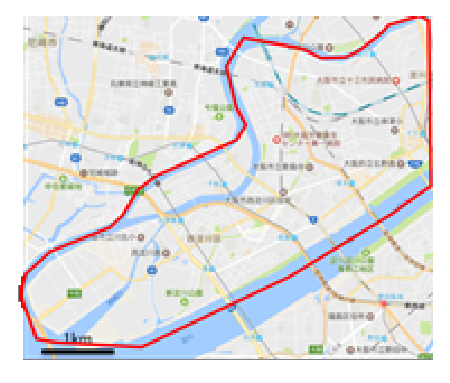
\includegraphics[width=.49\linewidth]{Figs.noda/figure-08.nishiyodogawa.eps}~
  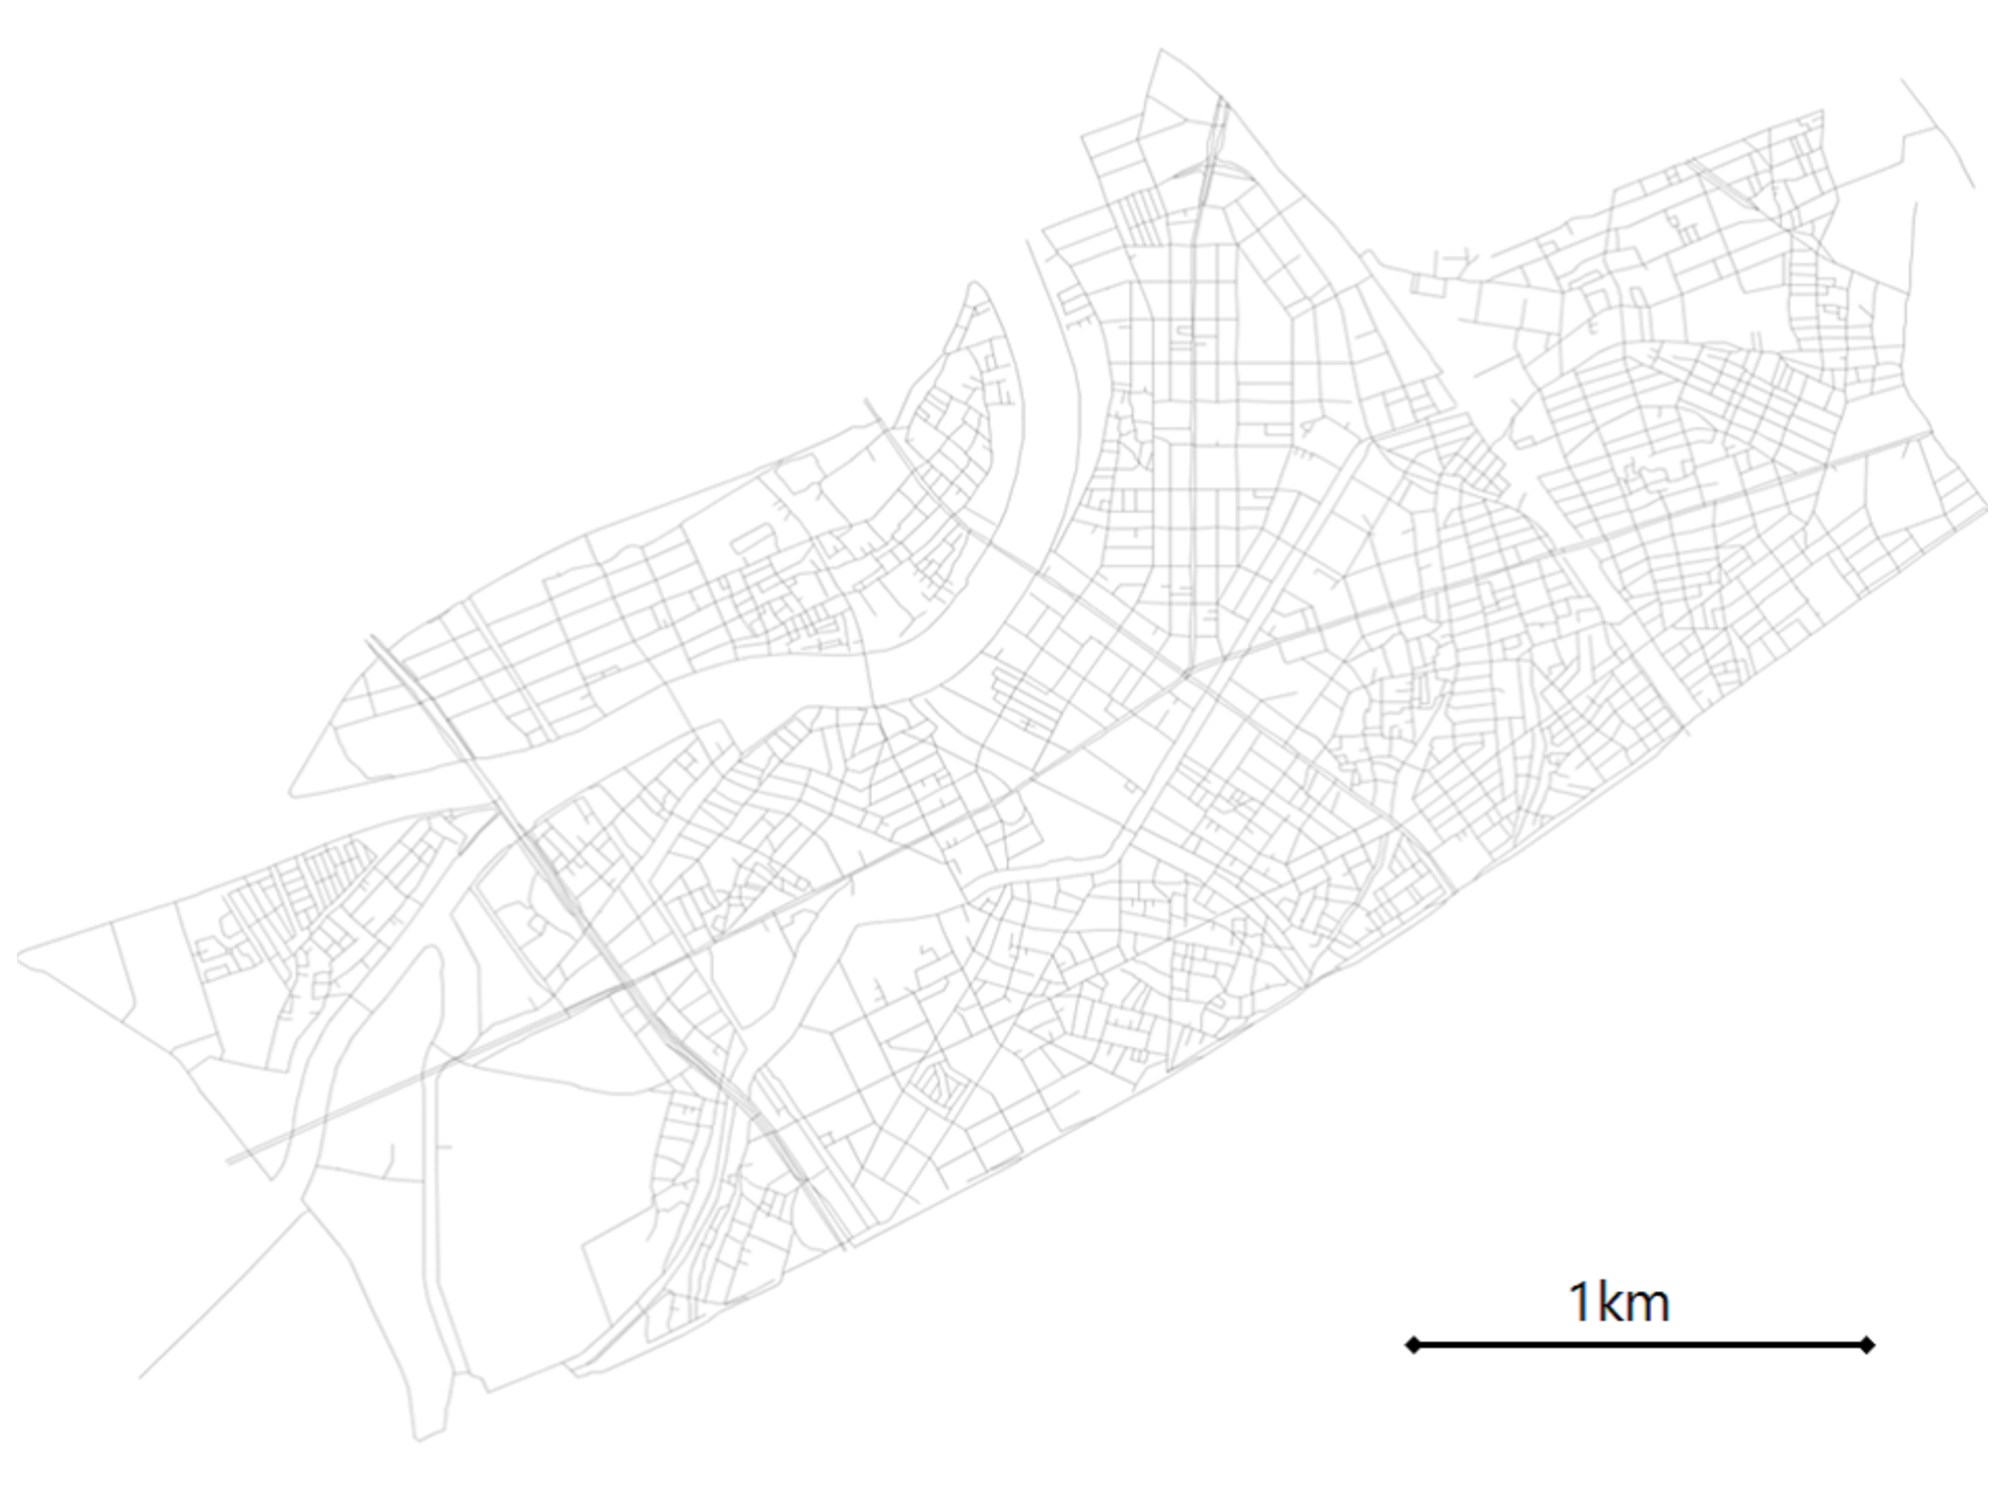
\includegraphics[width=0.49\linewidth]{Figs.noda/yodogawa_map}
  \caption{Nishiyodogawa Area (left) and
    Road Map (right) used in Pedestrian Simulation}
  \label{fig:Figs.noda/figure-08.nishiyodogawa.eps}
\end{figure}
%%++++++++++++++++++++++++++++++++++++++++++++++++++++++++++++++++++++++

%%------------------------------
\subsubsection{Multi-Objective Optimization}
\label{sss:moea}
%% - - - - - - - - - - - - - - -

As described before, evacuation planning is a dilemma
between evacuation time and simple-ness of evacuation rule.
From the viewpoint of the minimization of evacuation time,
it is better to use the result of mathematical optimization
like maximum network-flow \cite{kobayashi:2016}.
However, we need to guide large number of people that include
ones who are not acquainted with the place like visitors.
So, the guidance should be simple enough to understand and to follow easily.


In order to know the relationship of these two objectives,
we apply NSGA-II(Elitist Non-Dominated Sorting Genetic Algorithm)
\cite{deb:nsga}, a genetic algorithm for
multiple objective optimization\cite{deb:moea}.

For the first objection function, the evacuation time,
is estimated by simulation using CrowdWalk for each guidance plan.

For the second objective function, the simple-ness of evacuation plans,
we introduce `entropy' of the plan as follows.
The basic concept of the entropy
is illustrated in \figref{fig:Figs.noda/figure-09.evac_rule.eps}.
Suppose two connecting zones, $z_i$ and $z_j$ in the area, and
populations of the zones are $n_i$ and $n_j$, respectively.
If the two rules for these zones has same via point and destination,
then the entropy is zero.
Otherwise, 
the entropy of this pair is defined by:
\begin{eqnarray}
  H(z_i,z_j) & = & - (n_i/(n_i + n_j))\log(n_i/(n_i + n_j))
                  - (n_j/(n_i + n_j))\log(n_j/(n_i + n_j))
                  .
                  \nonumber
\end{eqnarray}
Finally, we use total entropy $H = \sum_{z_i,z_j} H(z_i, z_j)$
for the index of the complexity of the guidance (negative value
of the simple-ness).


%%++++++++++++++++++++++++++++++++++++++++++++++++++++++++++++++++++++++
\begin{figure}
  \centering
  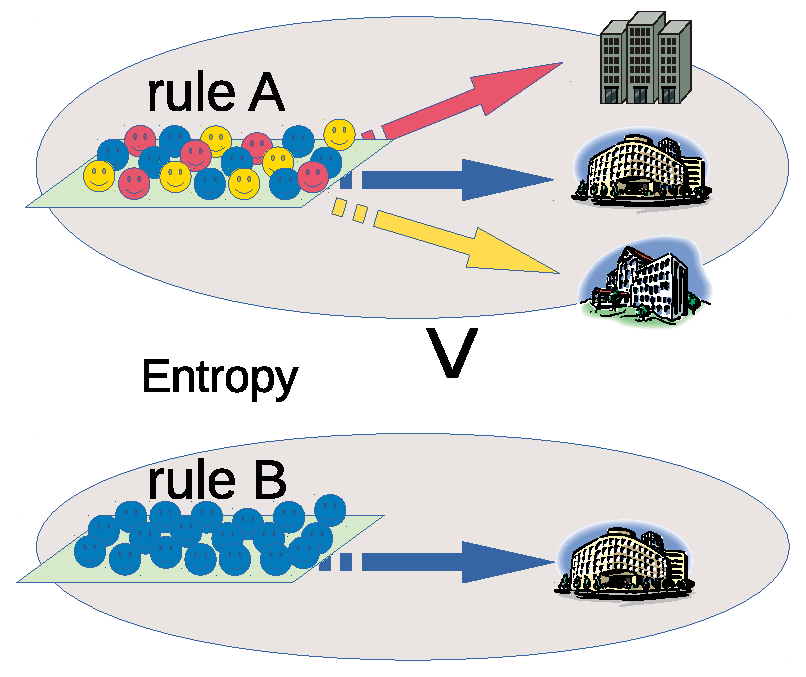
\includegraphics[width=.5\linewidth]{Figs.noda/figure-09.evac_rule.eps}
  \caption{Rule Entropy}
  \label{fig:Figs.noda/figure-09.evac_rule.eps}
\end{figure}
%%++++++++++++++++++++++++++++++++++++++++++++++++++++++++++++++++++++++

%%------------------------------
\subsubsection{Experimental Result and Discussion}
\label{sss:nsga-experiment}
%% - - - - - - - - - - - - - - -

In order to run NSGA-II for this evacuation plan,
we utilized OACIS\cite{murase:2014} to manage the large number of runs.
The search space of this problem is so huge
($R^{73} \times 533^{146} \times 86^{146}$)
and NSGA-II requires large number of populations (about 100--1,000).
So we need to run so many runs for the optimization.
In the experiment, we runs 500 generations with 100 population
for the optimization,
which means we run 500,000 simulations
\footnote{We runs 10 simulations for one evacuation plan
  to calculate average evacuation time.}
for this experiment.

To control NSGA-II procedure, we utilize the ruby plug-in facility of OACIS.
In the actual GA procedure, we use `simulated binary crossover' and
`polynomial mutation' for creating new generations,
and Paleto ranking mechanism to determine the selection.


\Figref{fig:Figs.noda/figure-11.evac_wide.eps} shows the result
of the experiment.
In this graph, vertical and horizontal axes indicate
evacuation time and the complexity of plan (total entropy
scaled by 100), respectively.
The color of the dot indicates the generations.
From this result,
we can see that the evacuation plans are improved by progress
of generations, and almost saturate to boundary of 3000 for
evacuation time and 2100 for complexity of guidance.
In order to minimize the evacuation time,
we need to choose relatively complex guidance (the complexity is about 2200
rather than 2100).
On the other hand, if we consider simplify the complexity,
the evacuation time increase drastically up to 7000.
And, we can see reasonable guidance will exist the most left-bottom
area of the Paleto front in this graph.

%%++++++++++++++++++++++++++++++++++++++++++++++++++++++++++++++++++++++
\begin{figure}
  \centering
  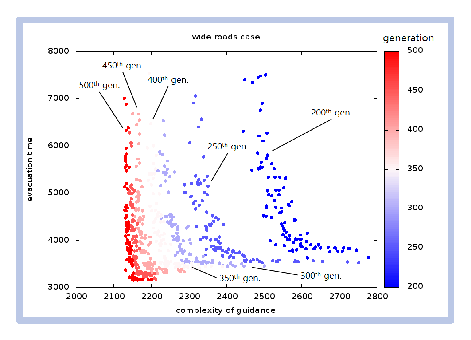
\includegraphics[width=.6\linewidth]{Figs.noda/figure-11.evac_wide.eps}
  \caption{Result of Evacuation Simulation (wide road)}
  \label{fig:Figs.noda/figure-11.evac_wide.eps}
\end{figure}
%%++++++++++++++++++++++++++++++++++++++++++++++++++++++++++++++++++++++

\Figref{fig:Figs.noda/figure-10.evac_narrow.eps} also
shows the result of the case that the people use only pedestrian road.
In this case, the boundary of the evacuation time increase to 4500,
but the complexity of guidance is similar to the previous case.

%%++++++++++++++++++++++++++++++++++++++++++++++++++++++++++++++++++++++
\begin{figure}
  \centering
  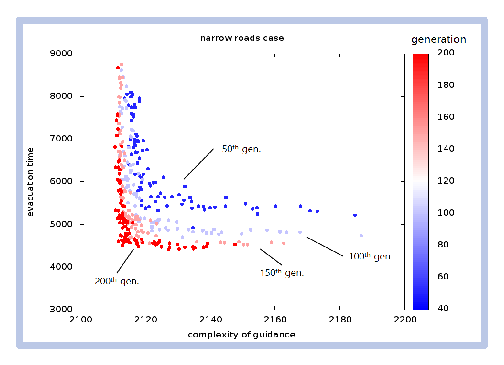
\includegraphics[width=.6\linewidth]{Figs.noda/figure-10.evac_narrow.eps}
  \caption{Result of Evacuation Simulation (narrow road)}
  \label{fig:Figs.noda/figure-10.evac_narrow.eps}
\end{figure}
%%++++++++++++++++++++++++++++++++++++++++++++++++++++++++++++++++++++++

As shown in this section,
evolutionary methods using OACIS can be a powerful tool
to investigate such social problems.
We also succeed to apply CARAVAN to run the same procedure
on K-computer.
This combination enables to run larger scale of simulations
and search spaces.


